\begingroup
\clearpage% Manually insert \clearpage
\let\clearpage\relax% Remove \clearpage functionality
\vspace*{-16pt}% Insert needed vertical retraction
\chapter[PRELIMINARY NON-AGNOSTIC BSM MODEL ANOMALY SEARCH]{PRELIMINARY NON-AGNOSTIC BSM MODEL ANOMALY SEARCH}
\endgroup

After the success of the agnostic anomaly detection search discussed in Chapter~\ref{ch6}, it was decided to try to adapt this technique to look for a specific \gls{bsm} signal. 
The frameworks for the anomaly detection were already set in place, all they needed was to be adjusted for a different analysis. This short chapter discusses \textbf{very preliminary} 
plots for another anomaly detection study. Unfortunately, this analysis started on the last part of my degree and I didn't have the time to properly obtain results.
Though, the frameworks have been adapted and preliminary anomaly detection studies were conducted. This analysis is expected to be continued by a graduate colleague after my 
graduation.

\section{SH $\rightarrow b\bar{b}b\bar{b}$ Anomaly Detection }

This is a search for a massive scalar boson that decays to a light scalar and a Higgs boson in the four b-quark boosted topology. This model expects a massive scalar boson X 
decay into a lighter scalar boson Y and a \gls{sm} Higgs boson H through the process X$\rightarrow$SH$\rightarrow b\bar{b}b\bar{b}$. This search uses proton-proton collision 
data taken by the \gls{atlas} detector during Run 2 at a \gls{cme} of 13 TeV corresponding to a luminosity of 138 $\textrm{fb}^{\textrm{-1}}$. The search is dedicated to 
a range of mass hypotheses. For the massive X scalar, a range of 0.3-6 TeV is set, and for the lighter Y scalar, the range of 70-5000 GeV. Both the lighter scalar and the 
\gls{sm} Higgs boson are Lorentz-boosted and therefore their b quark-antiquark pair are collimated and are reconstructed using a single large-R jet structure. The invariant mass 
of one pair of the b quark-antiquark pairs is required to be compatible with the Higgs boson of 125 GeV. The approach to find possible resonances and to set limits on these 
masses will be very similar to the previous anomaly detection technique that was applied in Chapter~\ref{ch6} for agnostic \gls{bsm} signals. 

\subsection{Event Selection}

Since the final topology requires 2 b quark-antiquark pairs, the ideal boosted large-R events contain two double b-tagged large-R jets. The choice of minimum $\textit{P}_{\textrm{T}}$ 
must be sufficient to contain the possibility of having a heaviest massive scalar boson mass hypotheses of 4 TeV. Due to the uniqueness of the required topology, it is crucial 
to ensure there is enough training statistics for a proper \gls{ml} model while also not biasing it on signal events. The minimum chosen $\textit{P}_{\textrm{T}}$ for the leading 
large-R jet is taken to be 450 Gev while the second leading large-R jet is required to have a minimum of 250 GeV ($\textit{P}_{\textrm{T}}$(j1(j2))$>$450(250) GeV), an 
$|\textrm{η}| < \textrm{2.0}$, and a jet mass of $\textrm{m}_j>$50 GeV. These large-R jets undergo a b-tagging criteria using the \gls{ftag} Xbb2020v3 tagger at the 70\% \gls{wp}.
This tagger is much like the DL1d tagger than can identify between b-, c-, and light-quarks up to a certain efficiency, but instead of a single quark, the Xbb tagger can 
identify large-R jets that may contain two b-jets up to a certain efficiency. These events that contain a single large-R jet that is double b-tagged as a 1bb-tagged and 
events with two large-R jets that are both double-tagged as 2bb-tagged (events may contain other non-b-tagged jets). Figure X shows the cutflow and the chosen \gls{nn} training sample statistics. 
Using events that just contain a single 1bb-tagged large-R jet would lead to insufficient statistics to train a proper \gls{ae} model, therefore the training sample was chosen 
using the $\textit{P}_{\textrm{T}}$(j1(j2))$>$450(250) GeV cut. 

\begin{figure}[ht]
    \centering
    \begin{subfigure}[h]{0.45\linewidth}
    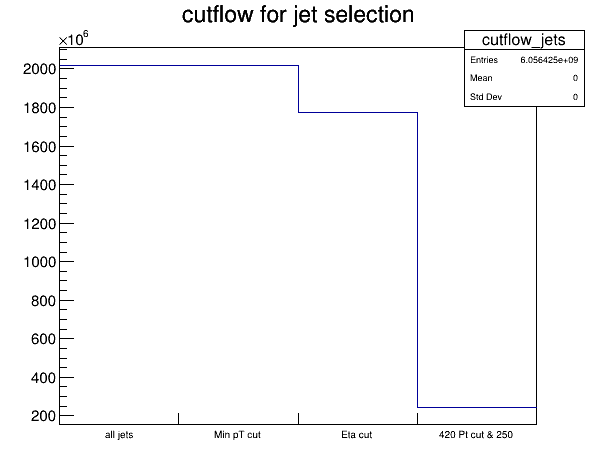
\includegraphics[scale=0.35]{figs/ch7/cutflow.png}%
    \caption{}
    \end{subfigure}
    \hfill
    \begin{subfigure}[h]{0.45\linewidth}
    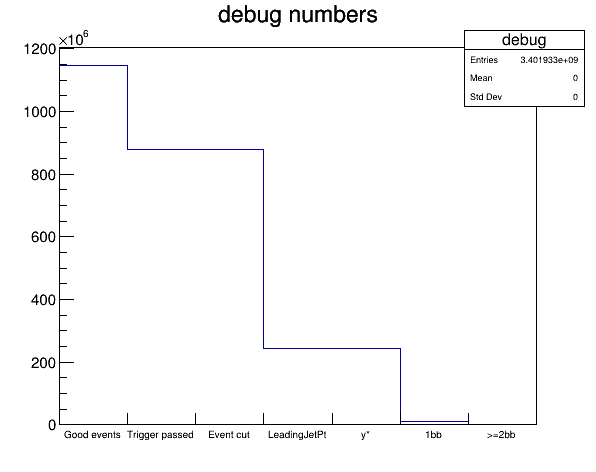
\includegraphics[scale=0.35]{figs/ch7/debug.png}%
    \caption{}
    \end{subfigure}
    \hfill
    \caption{(a) Shows the cutflow for Run 2 events. The last cut is on (j1(j2))$>$450(250) GeV. This cut equates to about 240M events. (b) Shows this 240M events that make the
             base cut and then shows how many are 1bb-tagged and 2bb-tagged. This equates to 1M events for 1bb-tagged and 6.2K for 2bb-tagged.}
\label{fig:sh4b-cutflow}
\end{figure}

\section{Event Representation}

Following the example in the anomaly detection analysis, a modified \gls{rmm} representation was chosen as the input to the deep-learning autoencoder (\gls{ae}) architecture. 
Since the events only contain \textit{x} amount of large-R jets and \textit{y} amount of double b-tagged large-R jets, the amount of input variables allowed within 
this representation decreases from the original layout. It was chosen to allow up to 5 large-R jets and up to 4 double b-tagged large-R jets. This layout contains a total 
of 100 input variables for the \gls{ae} (including one row and column of zeroes separating the large-R jets and the double b-tagged large-R jets). Figure X shows a diagram 
of this representation. The information layout is the same as the previous version discussed in Section~\ref{sec:evnt-input-rep}. Figure X shows two examples of this \gls{rmm}
representation. The left figure shows a single event containing three large-R jets and no double b-tagged large-R jets. The right plot shows all the events stacked into a single matrix.
This plot reveals there are events with 5 large-R jets. 

\begin{figure}[ht]
    \centering
    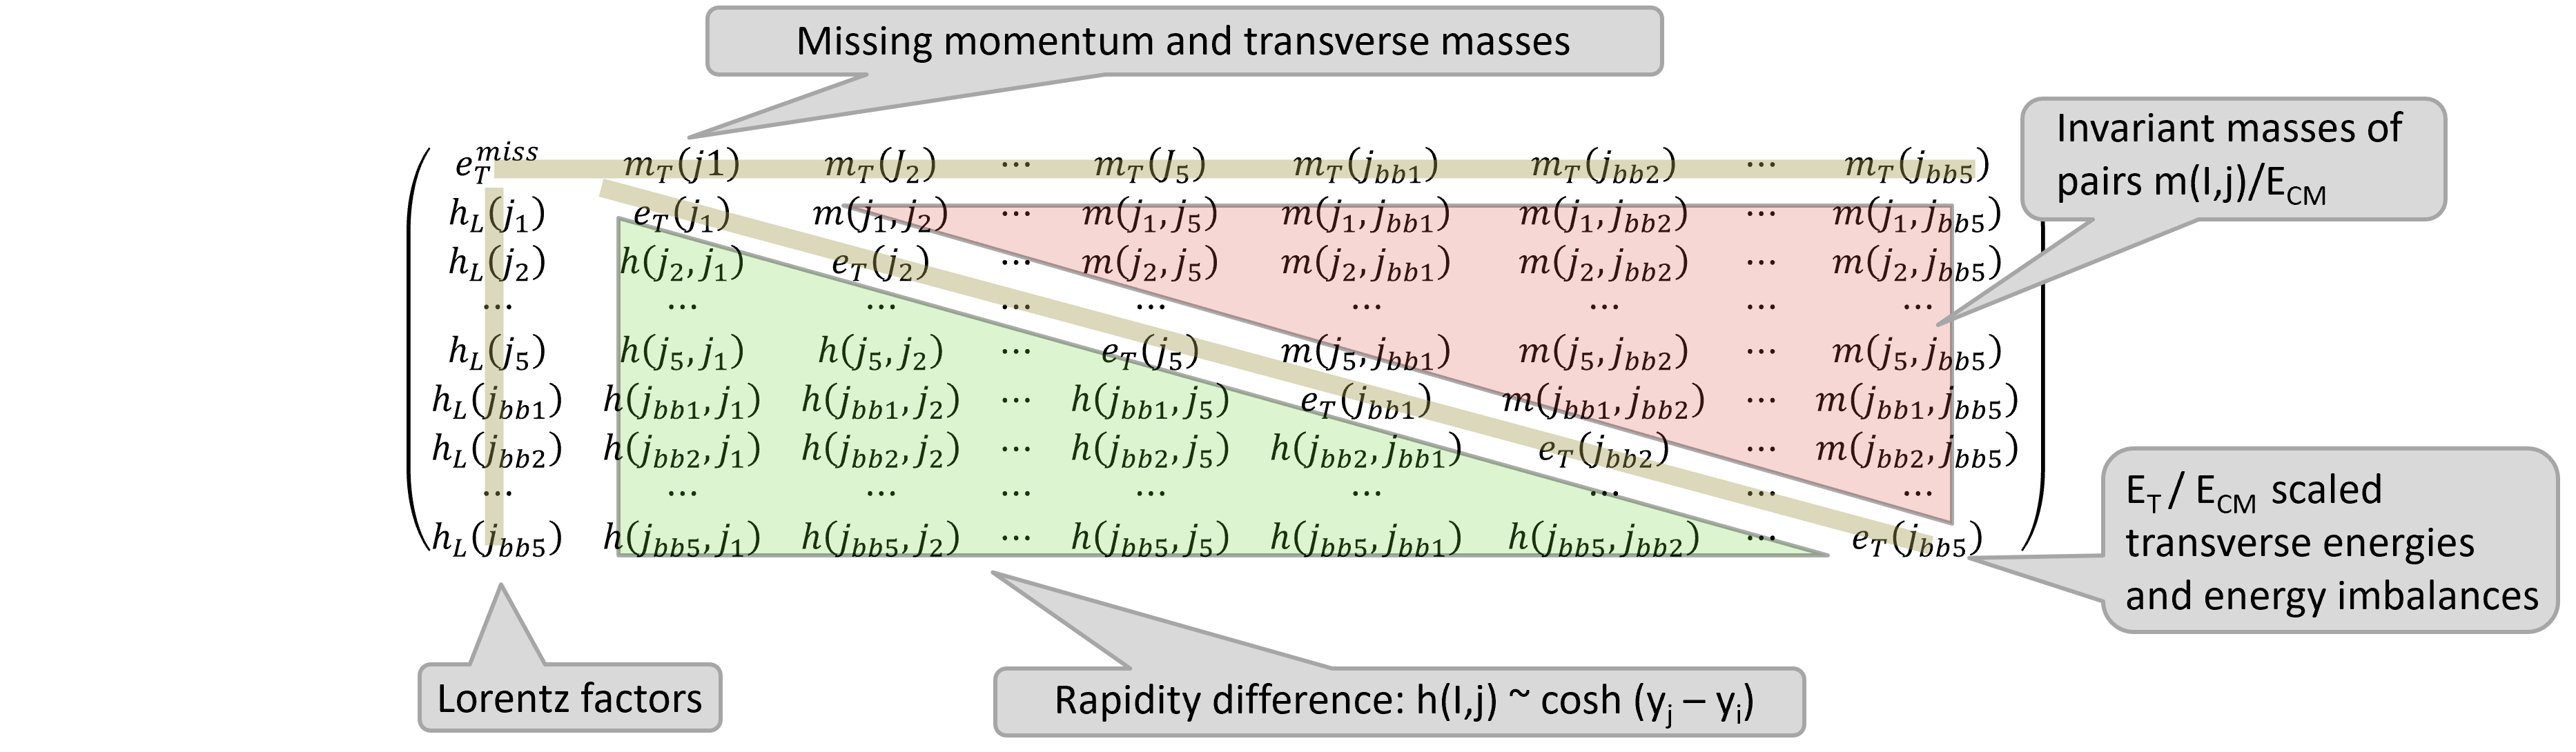
\includegraphics[scale=0.45]{figs/ch7/sh4b_rmm.png}%
    \caption{The Rapidity Mass Matrix representation for the SH $\rightarrow$ 4b analysis. This layout allows up to 5 large-R jets and 4 double b-tagged large-R jets. This 
    topology equates to 100 variables used for training the Autoencoder (included a row and column of zeroes).}
\label{fig:sh4b-rmm-diagram}
\end{figure}

\begin{figure}[ht]
    \centering
    \begin{subfigure}[h]{0.45\linewidth}
    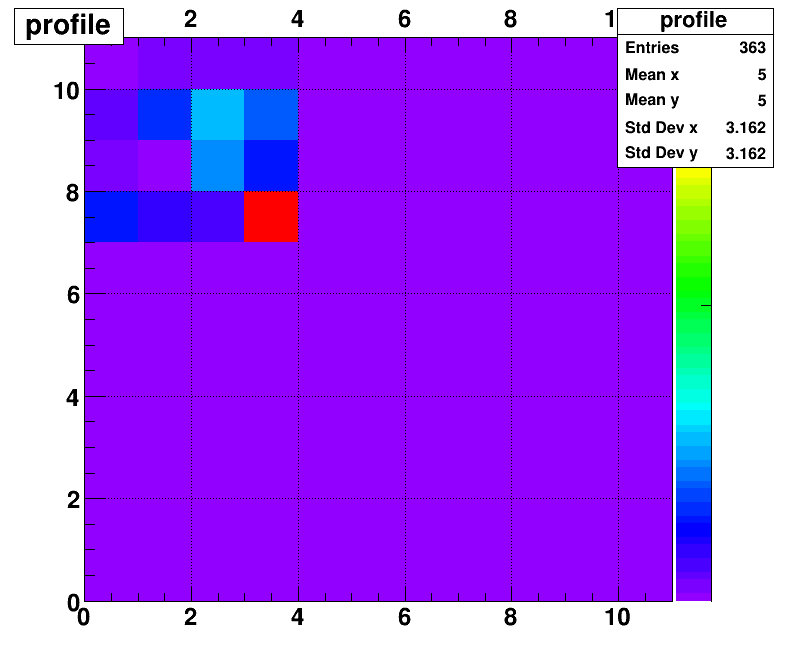
\includegraphics[scale=0.29]{figs/ch7/rmm_event.png}%
    \caption{}
    \end{subfigure}
    \hfill
    \begin{subfigure}[h]{0.45\linewidth}
    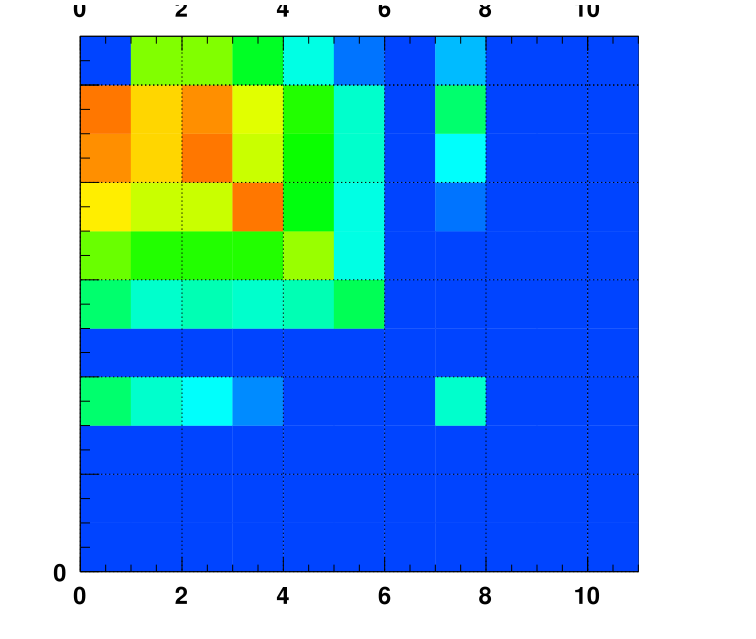
\includegraphics[scale=0.4]{figs/ch7/validate_data_0.png}%
    \caption{}
    \end{subfigure}
    \hfill
    \caption{(a) Shows a single event that contains three large-R jets using this new RMM representation. (b) Shows all the events stacked into a single RMM. This plot shows 
    there are events that contain 5 large-R jets. The row and column for the second double b-tagged large-R jet show to be almost empty, this is due to the fact that there are only 
    6.2K with respect to a total of 240M events shown in the first few rows and columns.}
\label{fig:sh4b-rmm-valid}
\end{figure}

\subsection{Autoencoder Training}

The preliminary \gls{ae} architecture can be seen in Figure~\ref{tab:ae-arch}. Just as previously discussed, this architecture contains an encoder, latent layer, and a decoder. This 
architecture compresses data from the input into the latent, then decompresses it using the decoder. The loss value calculated by the loss function is recorded and used 
for the anomaly score as the form of log(\textit{loss}). This model was training using 1\% of Run 2 large-R jet data, equating to 2.4M events with a 7:3 ratio for training 
and validation respectively. There requires many more studies in order to optimize this architecture but this was used for preliminary loss distribution studies. 

\begin{figure}[ht]
    \centering
    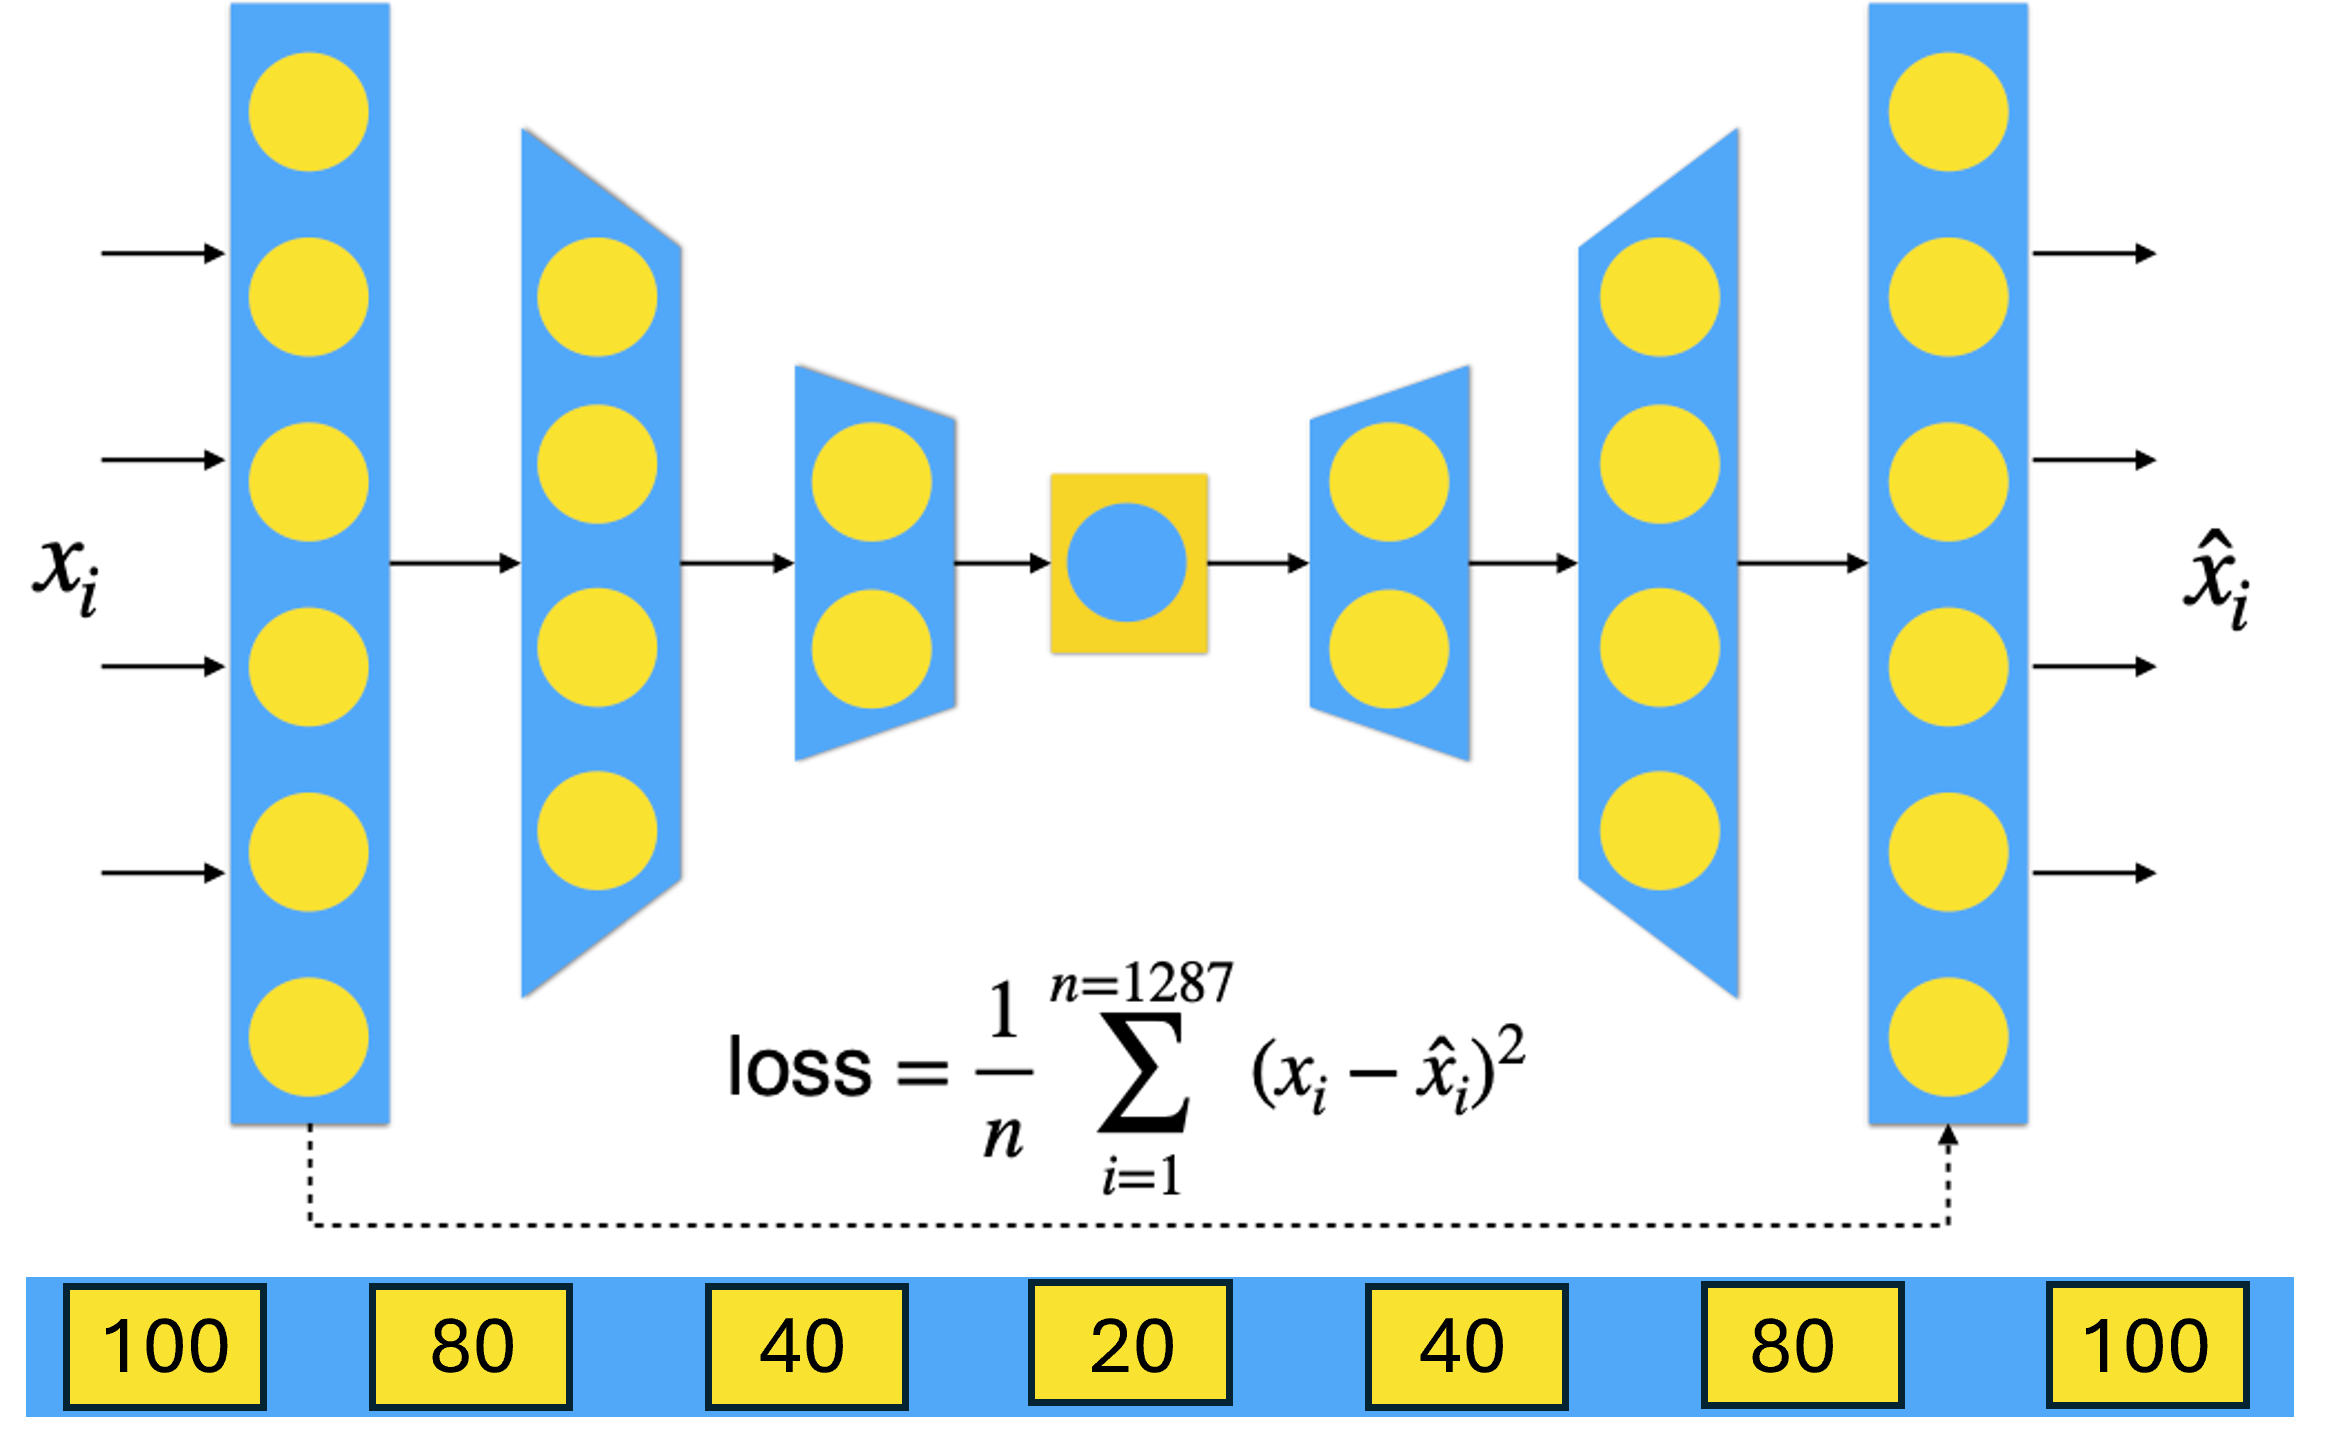
\includegraphics[scale=0.7]{figs/ch7/ae-arch.png}%
    \caption{Autoencoder architecture diagram for preliminary studies for the SH$\rightarrow$4b analysis. The first part of this architecture consists of an encoder that compresses 
    data into the latent layer, the decoder then decompresses the data and attempts to reconstruct the original input. The number of neural nodes are shown on the bottom.}
\label{fig:sh4b-ae-arch}
\end{figure}

\section{Preliminary Loss Distribution Studies}

The data sample contains a total of 240M events consisting of large-R jets with that made the cut of $\textit{P}_{\textrm{T}}$(j1(j2))$>$450(250) GeV. This dataset consists 
of the entire Run 2 data-taking campaign that was taken over the years of 2015-2018. This dataset was then split into their respective years and plotted in order to see if 
there are any year dependence due to pile-up conditions. This can be seen in Figure~\ref{fig:sh4b-year-dep} (the ratio plot needs to be adjusted).

\begin{figure}[ht]
    \centering
    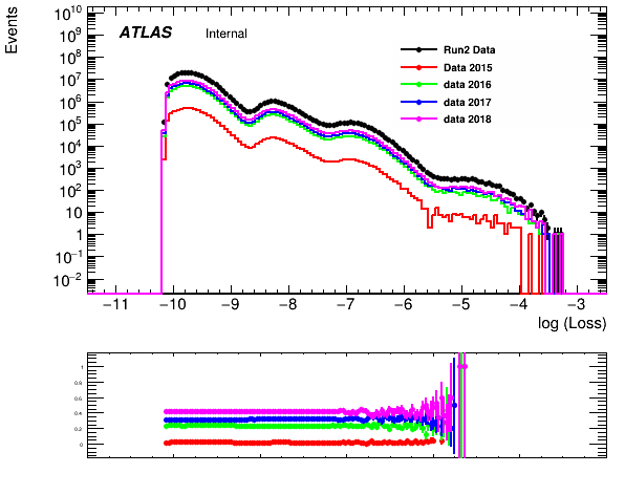
\includegraphics[scale=0.7]{figs/ch7/year-dep.png}%
    \caption{The log(\textit{loss}) distribution for all of Run 2 and its data-taking years. No yearly dependence is observed. The ratio plot needs to be adjusted}
\label{fig:sh4b-year-dep}
\end{figure}

The distribution in Figure~\ref{fig:sh4b-data-shapes} shows cascading of four peaks. This is due to the amount of objects allowed in the input representation. Figure X points out 
the origination of these peaks. The far most left peak is the least anomalous events which contain two large-R jets that are not double b-tagged. The second most left 
peak are events that contain three large-R jets. The third peak is then events that contain at least one large-R jet and one 1bb-tagged large-R jet. The final peak 
on the right is the events that contain 2bb-tagged large-R jets. There are other jets with odd combinations that do exist as can see in the validation \gls{rmm} plot on the 
right in Figure~\ref{fig:sh4b-rmm-valid} which are contained in or between these peaks. 
\newpage
\begin{figure}[ht]
    \centering
    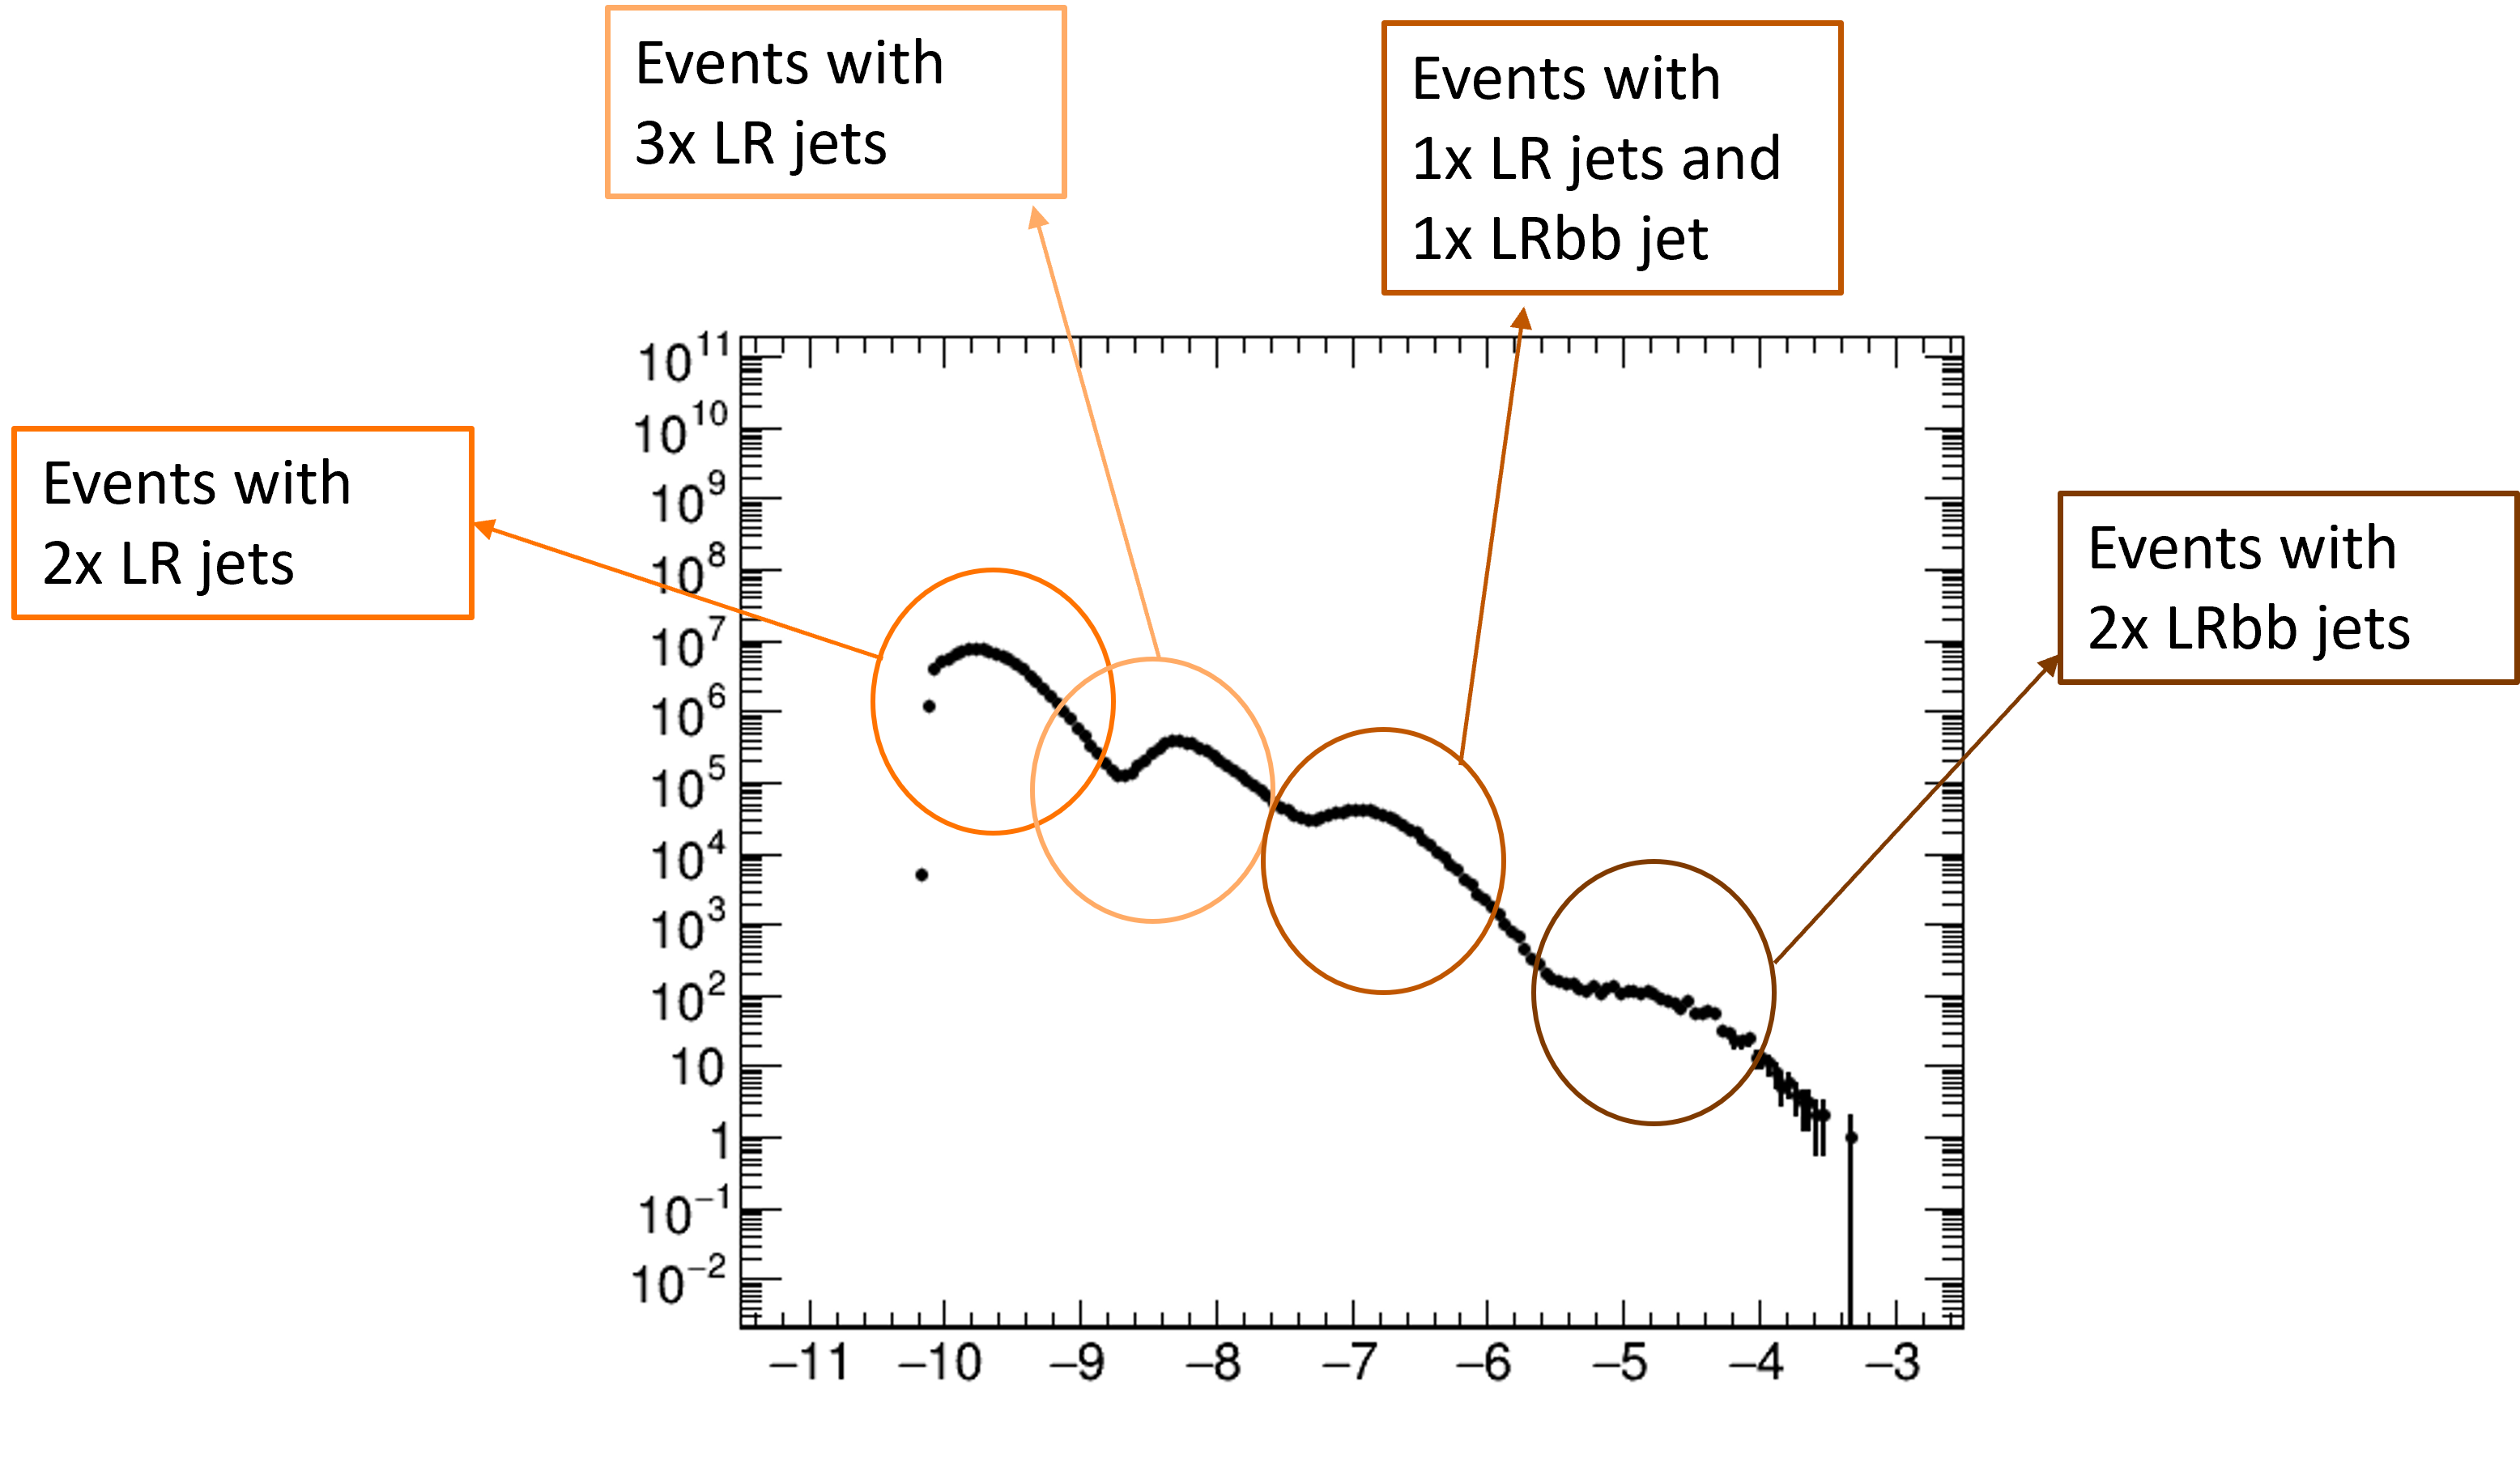
\includegraphics[scale=0.6]{figs/ch7/data-shapes.png}%
    \caption{Diagram of data log(\textit{loss}) distribution showing the origination of its four peaks.}
\label{fig:sh4b-data-shapes}
\end{figure}

There are six mass hypotheses for the large scalar boson and the light scalar boson that was chosen to help with benchmarking the \gls{ae} model. These six mass hypotheses are:

\begin{enumerate}
    \item Large Scalar Mass X: \textbf{1 TeV}, Light Scalar Mass S: \textbf{500 GeV}
    \item Large Scalar Mass X: \textbf{3 TeV}, Light Scalar Mass S: \textbf{750 GeV}
    \item Large Scalar Mass X: \textbf{300 GeV}, Light Scalar Mass S: \textbf{70 GeV}
    \item Large Scalar Mass X: \textbf{6 TeV}, Light Scalar Mass S: \textbf{1 TeV}
    \item Large Scalar Mass X: \textbf{6 TeV}, Light Scalar Mass S: \textbf{5 TeV}
    \item Large Scalar Mass X: \textbf{750 GeV}, Light Scalar Mass S: \textbf{250 GeV}
\end{enumerate}

The loss distributions of these six models along with data are seen in Figure~\ref{fig:sh4b-bsm-data-nolog}. These models are not scaled to their expected event count from Run 2 luminosity, but they 
do demonstrate the separation power of the \gls{ae}.


\begin{figure}[ht]
    \centering
    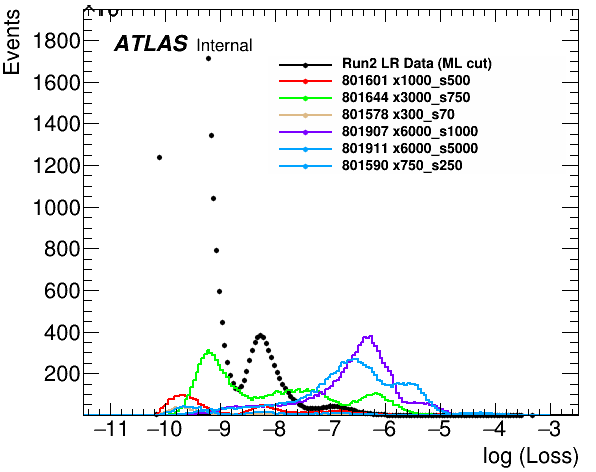
\includegraphics[scale=0.6]{figs/ch7/loss_data1percent_nolog_BSM.png}%
    \caption{Log(\textit{loss}) for Run 2 data and six mass hypothesis for the large scalar boson X and the lighter scalar boson S. The BSM events are not scaled to their expected 
    event count with respect to the luminosity. The y-axis is not log scaled.}
\label{fig:sh4b-bsm-data-nolog}
\end{figure}

\subsection{Preliminary Anomaly Region Definition}

The previous anomaly detection analysis used a calculated \gls{bsm} event count defined from the benchmark \gls{bsm} models used within the studies. That is one approach to 
define the anomaly region. The two definitions that are currently used (subject to change) are based on the double b-tagged event counts. The first \gls{ar} is of those 
that contain a single 1bb-tagged large-R jet. A second region is based on the event count of those that contain 2bb-tagged large-R jets. The \gls{ar}s that contain the 
correlated event counts can be seen in Figure X as a red line and pink dashed line. 

\newpage



\section{Conclusion}

These studies are still in the preliminary stage and should not be taken as any final result. This work is showing promise and should end in an interesting result, especially 
when it gets to set limits on the mass hypotheses. 
\par
There needs to be many more studies on the finding the optimized \gls{ae} architecture. Also, is the current chosen \gls{rmm} representation the best choice? Is it preferred 
to choose a topology that won't discriminate between the number of objects within the event? The \gls{bsm} models originally required to have 2bb-tagged large-R jets, so maybe 
this discrimination may work out best. Should the \gls{ar} cuts be based on the event counts of 1bb and 2bb-tagged large-R jets or should it be based on the event counts of the 
\gls{bsm} models themselves. \gls{mc} background events were simulated but not yet studied for this analysis which are crucial to start looking into the fit procedure. 
These are but a few tasks that need to be studied. 
\newpage
\begin{figure}[ht]
    \centering
    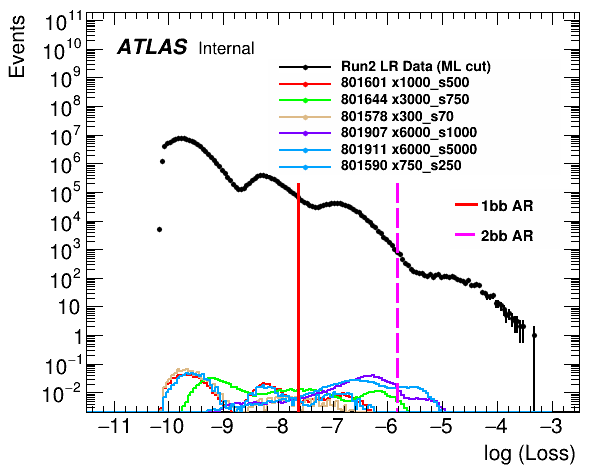
\includegraphics[scale=0.6]{figs/ch7/loss_data1percent_BSM.png}%
    \caption{Log(\textit{loss}) for Run 2 data and the six mass hypotheses. Two AR cuts are used to using the event count for 1bb-tagged large-R jets and 2bb-tagged large-R 
    jets. BSM models integrals are scaled to 1. The 1bb-tagged AR is seen as a red line and the 2bb AR is seen as a pink dashed line.}
\label{fig:sh4b-bsm-data-}
\end{figure}